\subsection{Dynamic K-Cycle}

\begin{frame}
	\begin{block}{Main idea}
		Compute the costs for all groups of variables with size up to $K$ and store them in a \alert{single} pattern database
	\end{block}
	\begin{figure}
		\centering
		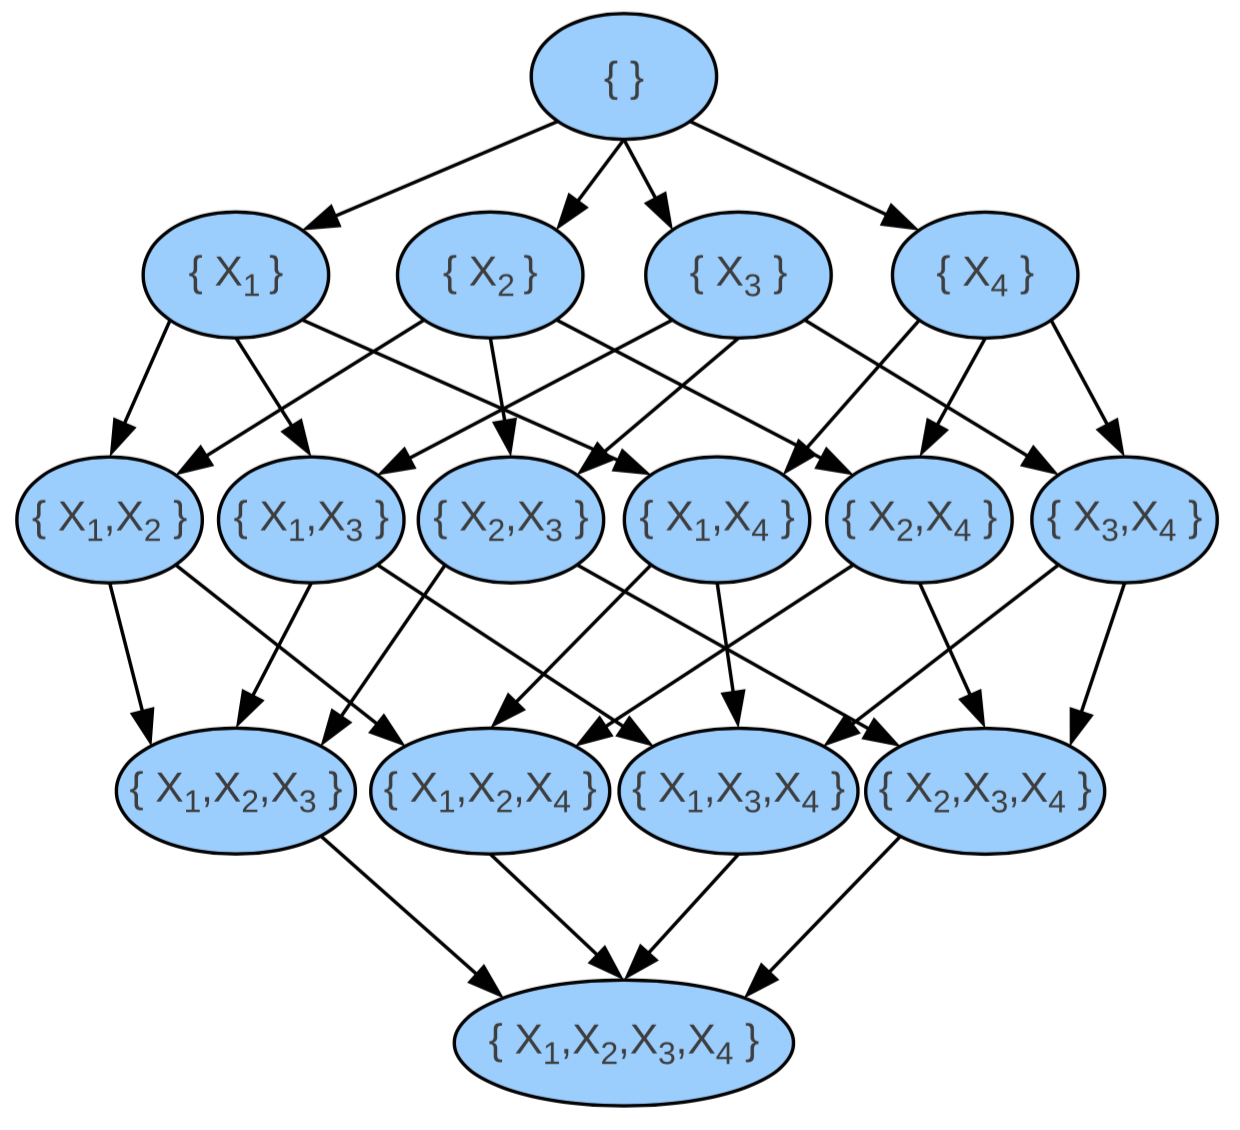
\includegraphics[height=4cm]{./images/order_graph}
	\end{figure}
\end{frame}

\begin{frame}
	\begin{block}{Theorem 3}
		The cost of the pattern $U$, $c( U )$, is equal to the shortest distance from $V \setminus U$ to the goal node in the order graph.
			\[ cost( U ) = shortest\_distance( V \setminus U ) \]
	\end{block}
	\begin{figure}
		\centering
		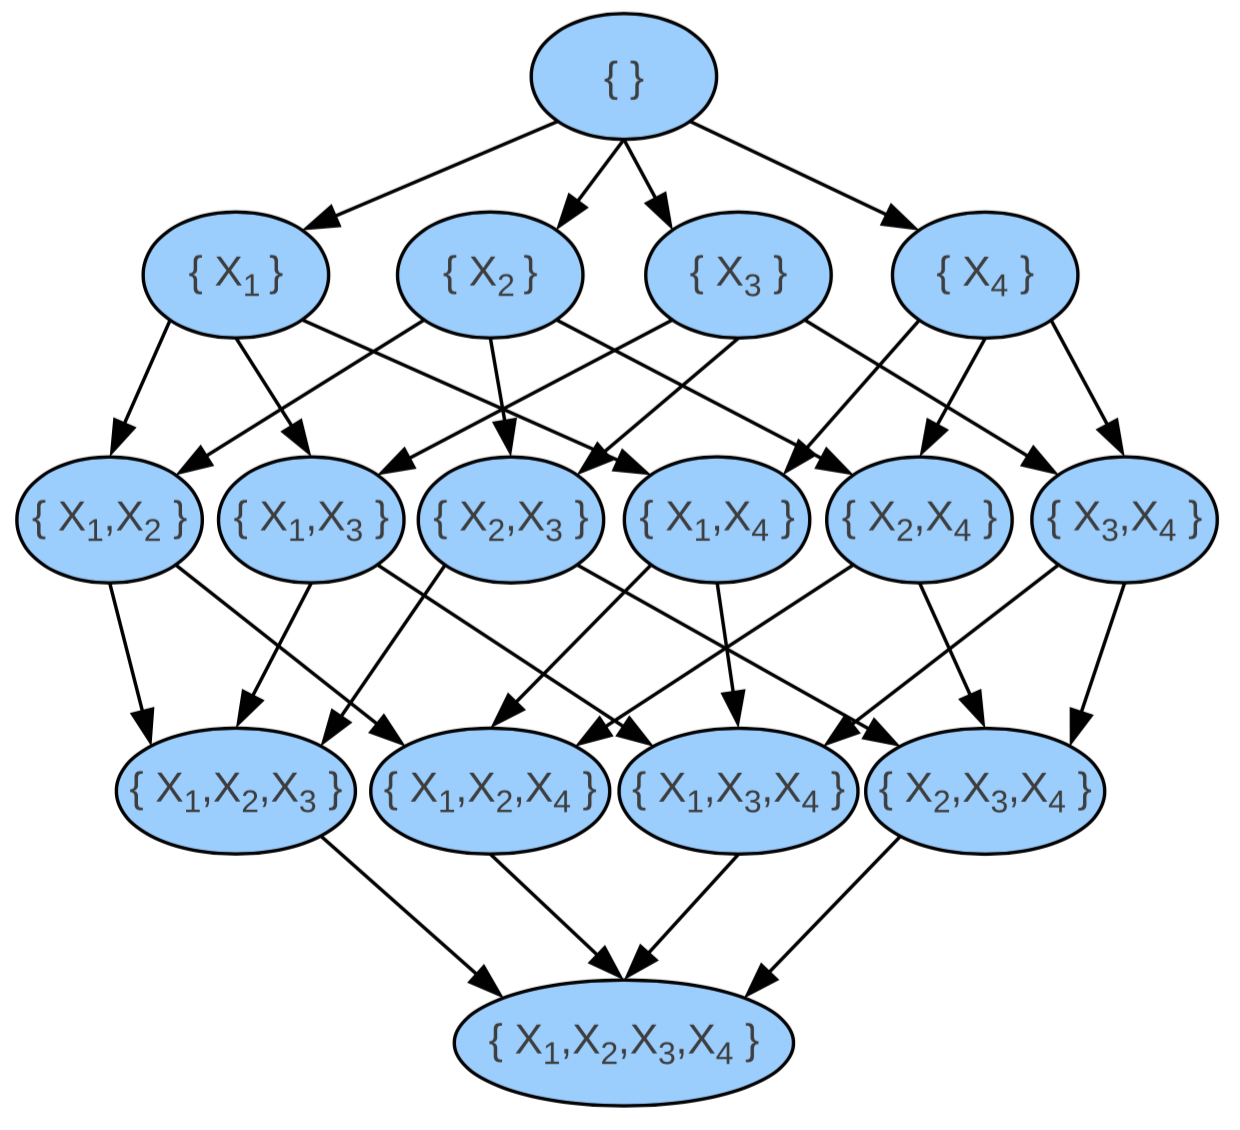
\includegraphics[height=4cm]{./images/order_graph}
	\end{figure}
\end{frame}

\begin{frame}
	The algorithm is as follows:
	\begin{itemize}
		\item Perform a breadth-first search in the last $K$ layers of order graph
		\begin{itemize}
			\item In each node $S$, update $shortest\_distance( S )$
			\item Calculate $diff( S )$, the difference between the cost and $h_{simple}$
			\item Prune $S$ if does not improve related to $h_{simple}$
			\item Set pattern $cost( V \setminus S ) = shortest\_distance( S )$
		\end{itemize}
		\item Sort patterns based on $diff( S )$ in descending order
	\end{itemize}
	\vskip2em
	\pause
	\begin{center}
		\large
		How do I calculate the heuristic \alert{$h_{dynamic}$}?
	\end{center}
\end{frame}

\begin{frame}
	\makeatletter
\def\BState{\State\hskip-\ALG@thistlm}
\makeatother

\begin{algorithm}[H]
	\scriptsize
	\DontPrintSemicolon
	$h \leftarrow 0$ \;
	$R \leftarrow U$ \;
	\For{each $S \in PD$}{
		\If{$S \subset R$}{
			$R \leftarrow R \setminus S$ \;
			$h \leftarrow h + PD( S )$
		}
	}
	return $h$
	\caption{$h_{dynamic}( U )$}
\end{algorithm}
	\pause
	\begin{center}
		\large
		Compute $h_{dynamic}$ is \alert{more expensive} than $h_{simple}$
	\end{center}
\end{frame}